\documentclass[11pt,a4paper]{article}

% ============================================================
% PACKAGES
% ============================================================
\usepackage[utf8]{inputenc}
\usepackage[T1]{fontenc}
\usepackage{geometry}
\usepackage{graphicx}
\usepackage{xcolor}
\usepackage{fancyhdr}
\usepackage{titlesec}
\usepackage{booktabs}
\usepackage{array}
\usepackage{tabularx}
\usepackage{hyperref}
\hypersetup{
	hidelinks
}
\usepackage{amsmath}
\usepackage{amssymb}
\usepackage{listings}
\usepackage{tikz}
\usepackage{float}

\geometry{
	a4paper,
	top=2.5cm, bottom=2.5cm,
	left=2.5cm, right=2.5cm,
	headheight=14pt
}

% ============================================================
% COLORS
% ============================================================
\definecolor{darkblue}{RGB}{0, 51, 102}
\definecolor{darkgray}{RGB}{60, 60, 60}
\definecolor{lightgray}{RGB}{220, 220, 220}
\definecolor{codeblue}{RGB}{30, 90, 150}
\definecolor{akashcolor}{RGB}{0, 100, 150}

% ============================================================
% LISTINGS
% ============================================================
\lstset{
	basicstyle=\ttfamily\small,
	breaklines=true,
	backgroundcolor=\color{lightgray},
	frame=single,
	framerule=0pt,
	numbers=none,
	keywordstyle=\color{codeblue}\bfseries,
	commentstyle=\color{darkgray},
	stringstyle=\color{darkblue},
	showstringspaces=false,
	language=bash,
	morekeywords={hpc, run, run-script}
}

% ============================================================
% STYLES
% ============================================================
\pagestyle{fancy}
\fancyhf{}
\fancyhead[L]{\textbf{Zest}}
\fancyhead[R]{\small White Paper v1.0}
\fancyfoot[C]{\small\thepage}
\renewcommand{\headrulewidth}{0.5pt}

\titleformat{\section}
{\color{darkblue}\Large\bfseries}
{\thesection}{1em}{}[{\vspace{0.2cm}\noindent\color{lightgray}\hrule height 0.5pt}]

\titleformat{\subsection}
{\color{darkblue}\large\bfseries}
{\thesubsection}{0.8em}{}

\titleformat{\subsubsection}
{\color{darkgray}\bfseries}
{\thesubsubsection}{0.8em}{}

\titlespacing{\section}{0pt}{1.2cm}{0.6cm}
\titlespacing{\subsection}{0pt}{0.8cm}{0.4cm}

% ============================================================
% COMMANDS
% ============================================================
\newcommand{\highlight}[1]{\textbf{\color{darkblue}#1}}
\newcommand{\keypoint}[2]{%
	\vspace{0.4cm}
	\noindent\fcolorbox{darkblue}{white}{%
		\begin{minipage}{\dimexpr\linewidth-2\fboxsep-2\fboxrule}
			\vspace{0.1cm}
			{\small\color{darkblue}\textbf{#1}} \quad {\small #2}
			\vspace{0.1cm}
		\end{minipage}%
	}
	\vspace{0.4cm}
}

% ============================================================
% DOCUMENT
% ============================================================
\begin{document}
	
	% ============================================================
	% COVER PAGE
	% ============================================================
	\thispagestyle{empty}
	\vspace*{2cm}
	
	\begin{center}
		{\Huge\color{darkblue}\textbf{Zest}}
		\vspace{0.5cm}
		
		{\Large\color{darkgray}Simplified Scientific Computing on Distributed Infrastructure}
		\vspace{2cm}
		
		{\large\color{darkgray}\textit{Execute scientific tools on HPC/cloud infrastructure}}
		\vspace{0.2cm}
		
		{\large\color{darkgray}\textit{with a single command}}
		\vspace{3cm}
		
		{\large\color{darkgray}White Paper --- Version 1.0}
		\vspace{0.5cm}
		
		{\small\color{darkgray}Status: Early Development}
		\vspace{3cm}
		
		{\small\color{darkgray}Akash Network, Open Source CLI}
	\end{center}
	
	\vfill
	
	\noindent\color{darkgray}\small
	\textbf{Target Audience:} CNES, Aix-Marseille University, CMA CGM, Scientific Communities
	
	\newpage
	
	% ============================================================
	% TABLE OF CONTENTS
	% ============================================================
	\tableofcontents
	
	\newpage
	
	% ============================================================
	% SECTION 1: EXECUTIVE SUMMARY
	% ============================================================
	\section{Executive Summary}
	
	\highlight{Zest} is an open-source CLI tool designed to simplify the execution of scientific workloads on distributed infrastructure (Akash Network, traditional HPC, cloud).
	
	The goal: \textit{eliminate the complexity} associated with containerization, environment configuration, and file transfers.
	
	\subsection{The Problem}
	
	Researchers and engineers running intensive scientific pipelines face:
	
	\begin{itemize}
		\item Manual configuration of Docker/VMs
		\item Complex file transfer management
		\item Learning multiple tools (AWS CLI, Slurm, etc.)
		\item Infrastructure administration that consumes valuable time
		\item Vendor lock-in with single cloud providers
	\end{itemize}
	
	\subsection{The Solution}
	
	A single CLI interface, \highlight{tool-centric}, that:
	
	\begin{itemize}
		\item Hides infrastructure complexity
		\item Automates transfer, provisioning, and cleanup
		\item Supports pre-packaged tools (bioinformatics, geospatial) and custom scripts
		\item Works on decentralized (Akash) or traditional infrastructure
		\item Remains fully open-source and extensible
	\end{itemize}
	
	\subsection{Benefits for Researchers and Enterprises}
	
	\subsubsection{For Researchers}
	
	\begin{itemize}
		\item \textbf{Accelerated Research}: Less time on infrastructure, more on science. Move from idea to results in minutes, not weeks.
		\item \textbf{Reproducible Science}: Containerized tools ensure consistent execution environments across institutions.
		\item \textbf{Global Collaboration}: Shared tool registry enables seamless collaboration between international research teams.
		\item \textbf{Access to HPC}: Democratizes access to high-performance computing for researchers worldwide.
	\end{itemize}
	
	\subsubsection{For Enterprises}
	
	\begin{itemize}
		\item \textbf{Cost Optimization}: Pay only for compute resources used, with no upfront infrastructure investment.
		\item \textbf{Operational Efficiency}: Eliminates DevOps overhead for scientific workloads.
		\item \textbf{Scalability}: Easily scale compute resources up or down based on project needs.
		\item \textbf{Innovation Acceleration}: Focus on core business while leveraging external HPC resources.
	\end{itemize}
	
	\subsubsection{For the Global Scientific Community}
	
	\begin{itemize}
		\item \textbf{Democratization of Computing}: Researchers in developing countries can access world-class infrastructure without massive capital investment.
		\item \textbf{Decentralized Infrastructure}: Akash Network distributes computing globally, reducing geopolitical dependencies and local costs.
		\item \textbf{Reproducible Science}: Open-source code + public CLI = total transparency. Everyone can verify, reproduce, and improve.
		\item \textbf{Global Community}: Creates links between resource-rich institutions and labs with limited resources. Enables frictionless sharing of scientific pipelines.
		\item \textbf{Sustainable Impact}: Free and accessible tools = more inclusive science, more robust results (global peer review).
	\end{itemize}
	
	\keypoint{Free CLI + Managed Service}{The CLI is open-source and free. An optional web service will offer job management, history, multi-user support, and institutional integration.}
	
	\newpage
	
	% ============================================================
	% SECTION 2: TECHNICAL ARCHITECTURE
	% ============================================================
	\section{Technical Architecture}
	
	\subsection{Overview}
	
	HPC Flow operates on a simple three-layer architecture:
	
	\begin{figure}[H]
		\centering
		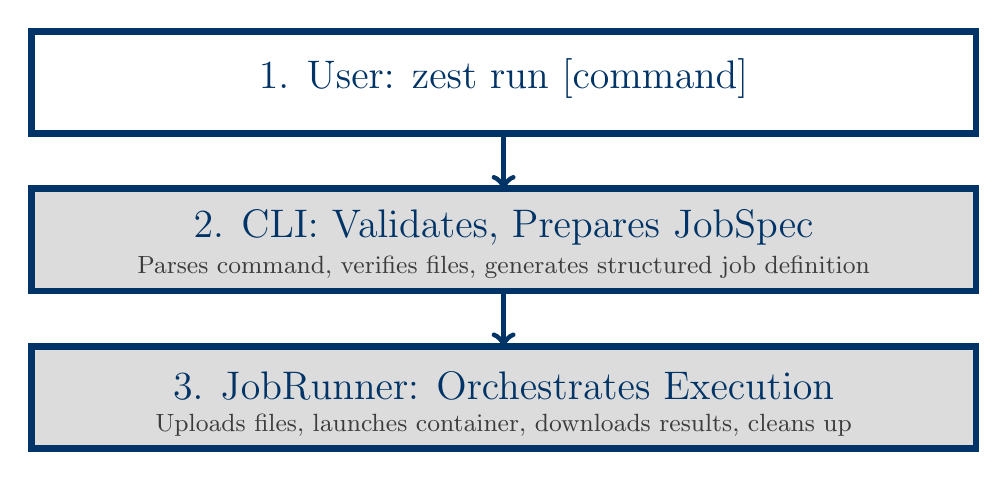
\begin{tikzpicture}[scale=1.0]
			
			% LAYER 1: USER
			\draw[darkblue, fill=white, line width=2.5] (-2, 7.5) rectangle (10, 8.8);
			\node[darkblue, font=\bfseries, font=\Large] at (4, 8.2) {1. User: zest run [command]};
			
			% ARROW
			\draw[->, line width=2, darkblue] (4, 7.5) -- (4, 6.8);
			
			% LAYER 2: CLI
			\draw[darkblue, fill=lightgray, line width=2.5] (-2, 5.5) rectangle (10, 6.8);
			\node[darkblue, font=\bfseries, font=\Large] at (4, 6.3) {2. CLI: Validates, Prepares JobSpec};
			\node[darkgray, font=\small] at (4, 5.8) {Parses command, verifies files, generates structured job definition};
			
			% ARROW
			\draw[->, line width=2, darkblue] (4, 5.5) -- (4, 4.8);
			
			% LAYER 3: JOBRUNNER
			\draw[darkblue, fill=lightgray, line width=2.5] (-2, 3.5) rectangle (10, 4.8);
			\node[darkblue, font=\bfseries, font=\Large] at (4, 4.3) {3. JobRunner: Orchestrates Execution};
			\node[darkgray, font=\small] at (4, 3.8) {Uploads files, launches container, downloads results, cleans up};
			
		\end{tikzpicture}
		\caption{Simplified Execution Flow}
	\end{figure}
	
	\subsection{Key Components}
	
	\subsubsection{1. CLI Layer}
	
	The Command-Line Interface (CLI) is the primary user interaction point. It:
	
	\begin{itemize}
		\item Parses user commands (e.g., \texttt{zest run vsearch --input data.fasta})
		\item Validates input files and parameters
		\item Constructs a \highlight{JobSpec} (structured job definition)
		\item Selects the appropriate backend (Akash, AWS, Slurm, etc.)
		\item Submits the job to the JobRunner
	\end{itemize}
	
	\subsubsection{2. JobSpec Definition}
	
	A structured YAML/JSON document defining:
	
	\begin{lstlisting}
		tool: vsearch
		version: "2.21.1"
		input_files:
		- metagenome_1M_reads.fasta
		output_files:
		- centroids.fasta
		parameters:
		id: 0.97
		threads: 16
		runtime: "docker://quay.io/biocontainers/vsearch:2.21.1"
		backend: akash
	\end{lstlisting}
	
	\subsubsection{3. JobRunner Abstraction}
	
	The core abstraction that handles backend-specific execution:
	
	\begin{lstlisting}
		class JobRunner(ABC):
		@abstractmethod
		def submit(self, job_spec: JobSpec) -> str:
		"""Submit job to backend and return job_id"""
		pass
		
		@abstractmethod
		def monitor(self, job_id: str) -> str:
		"""Monitor job execution and return status"""
		pass
		
		@abstractmethod
		def download(self, job_id: str, local_path: str) -> None:
		"""Download output files (job_id) -> local_files"""
		pass
		
		@abstractmethod
		def cleanup(self, job_id: str) -> None:
		"""Clean up backend resources"""
		pass
	\end{lstlisting}
	
	\subsubsection{4. Backend Implementations}
	
	\textbf{Phase 1 (MVP):} AkashJobRunner
	\begin{itemize}
		\item Uploads input files to Akash
		\item Creates an Akash deployment with the tool image
		\item Monitors execution via Akash logs
		\item Downloads results
		\item Destroys the deployment
	\end{itemize}
	
	\textbf{Phase 2+:} AWS, GCP, OVH, Slurm Support
	\begin{itemize}
		\item \textbf{AWSJobRunner}: Uses Lambda or EC2
		\item \textbf{GCPJobRunner}: Uses Cloud Run or Compute Engine
		\item \textbf{SlurmJobRunner}: Integrates with traditional HPC
	\end{itemize}
	
	\subsubsection{5. Custom Script Execution}
	
	For scientists with specific pipelines:
	
	\begin{lstlisting}
		zest run-script my_analysis.py \
		--runtime python:3.11 \
		--input data.csv \
		--output result.html \
		--cloud akash
	\end{lstlisting}
	
	The script and its dependencies (\texttt{requirements.txt}) are uploaded and executed in a base runtime.
	
	\newpage
	
	% ============================================================
	% SECTION 3: EXECUTION WORKFLOW
	% ============================================================
	\section{Execution Workflow}
	
	\subsection{Flow of a \texttt{hpc run} Command}
	
	\begin{enumerate}
		\item \textbf{Parsing}: CLI interprets the command and flags
		
		\item \textbf{Validation}: Checks file existence, flag validity, available resources
		
		\item \textbf{JobSpec Construction}: Creates a structured job description
		
		\item \textbf{Backend Selection}: Chooses the JobRunner (Akash, AWS, etc.)
		
		\item \textbf{Resource Provisioning}: Allocates resources on the backend
		
		\item \textbf{File Upload}: Transfers input files to remote
		
		\item \textbf{Job Execution}: Launches the container with arguments
		
		\item \textbf{Monitoring}: Polls status, captures logs
		
		\item \textbf{Result Download}: Retrieves output files locally
		
		\item \textbf{Cleanup}: Destroys the deployment
	\end{enumerate}
	
	\textbf{Total Duration:} A few seconds (provisioning) + compute time + a few seconds (download).
	
	\newpage
	
	% ============================================================
	% SECTION 4: TARGET USE CASES
	% ============================================================
	\section{Target Use Cases}
	
	\subsection{Bioinformatics}
	
	\subsubsection{Sequence Analysis (CNES, Universities)}
	
	Evolutionary biology researchers need clustering of thousands of DNA sequences.
	
	\begin{lstlisting}
		zest run vsearch \
		--input metagenome_1M_reads.fasta \
		--id 0.97 \
		--threads 16 \
		--output centroids.fasta \
		--cloud akash
	\end{lstlisting}
	
	\textbf{Advantage:} One command. No infrastructure administration.
	
	\subsubsection{BLAST / Alignment (Biotech, University)}
	
	\begin{lstlisting}
		zest run blast \
		--query proteins.fasta \
		--db nr \
		--output results.tsv \
		--cloud akash
	\end{lstlisting}
	
	\subsection{Geospatial}
	
	\subsubsection{DEM Raster Processing (CNES, CMA CGM Logistics)}
	
	Calculating slopes, aspects, vegetation indices on satellite imagery.
	
	\begin{lstlisting}
		zest run geoprocess \
		--input dem_region.tif \
		--operation slope \
		--output slope_map.tif \
		--cloud akash
	\end{lstlisting}
	
	\textbf{CMA CGM Use Case:} Logistics optimization via terrain relief analysis for route planning.
	
	\subsection{Custom Scripts}
	
	\subsubsection{Proprietary Data Analysis}
	
	Researcher with a specific pipeline (combination of in-house tools + standard libraries).
	
	\begin{lstlisting}
		zest run-script proprietary_analysis.py \
		--runtime python:3.11 \
		--input confidential_data.csv \
		--output report.html \
		--cloud akash
	\end{lstlisting}
	
	The \texttt{requirements.txt} file is automatically downloaded.
	
	\newpage
	
	% ============================================================
	% SECTION 5: AKASH NETWORK --- PRIMARY BACKEND
	% ============================================================
	\section{Akash Network: Primary Backend and Multi-Cloud Strategy}
	
	\subsection{What is Akash Network?}
	
	Akash Network is a decentralized cloud computing marketplace built on blockchain technology. Unlike traditional cloud providers (AWS, Google Cloud, Azure), Akash operates as an open marketplace where computing resources are traded peer-to-peer.
	
	Key characteristics:
	\begin{itemize}
		\item \textbf{Decentralized}: No single entity controls the infrastructure
		\item \textbf{Open Market}: Providers compete to offer resources, ensuring transparent pricing
		\item \textbf{Blockchain-Based}: Smart contracts automate resource allocation and payment
		\item \textbf{Container-First}: Native support for Docker containers
	\end{itemize}
	
	\subsection{Why Akash for Scientific Computing?}
	
	\begin{table}[H]
		\centering
		\small
		\begin{tabularx}{\linewidth}{l | c | c | c}
			\toprule
			\textbf{Criteria} & \textbf{Akash} & \textbf{AWS} & \textbf{GCP} \\
			\midrule
			Decentralized & $\checkmark$ & $\times$ & $\times$ \\
			60-80\% Cheaper & $\checkmark$ & Baseline & $\approx$ AWS \\
			No Vendor Lock-in & $\checkmark$ & $\times$ & $\times$ \\
			Open Market (peer-to-peer) & $\checkmark$ & $\times$ & $\times$ \\
			Easy Container Integration & $\checkmark$ & $\checkmark$ & $\checkmark$ \\
			\bottomrule
		\end{tabularx}
		\caption{Akash vs. Centralized Cloud Comparison}
	\end{table}
	
	\paragraph{1. Decentralization and Sovereignty}
	Akash is a decentralized blockchain. No single actor controls the infrastructure. Ideal for:
	\begin{itemize}
		\item \textbf{CNES}: No geopolitical dependencies for spatial data
		\item \textbf{CMA CGM}: Sensitive logistics data not centralized
		\item \textbf{Universities}: Flexible data governance
	\end{itemize}
	
	\paragraph{2. Cost Efficiency}
	Prices \textbf{60-80\% lower} than AWS/GCP due to the peer-to-peer model. Providers on Akash optimize their costs.
	
	\paragraph{3. No Vendor Lock-in}
	Multi-backend architecture allows switching to another cloud without changing user code. Sustainable competitive advantage.
	
	\paragraph{4. Open Market}
	Multiple providers bid for jobs. Price transparency. No captive pricing.
	
	\subsection{Akash Network Current Limitations and Roadmap}
	
	Akash Network is evolving with several major improvements planned:
	
	\begin{itemize}
		\item \textbf{Enhanced GPU Support}: Advanced support for NVIDIA H100, A100, and H200 GPUs with performance optimization for AI/ML and intensive computing
		
		\item \textbf{Improved SLA Guarantees}: Implementation of formal, automated SLA guarantees for better deployment reliability
		
		\item \textbf{Decentralized Storage Solution}: Deployment of an S3-compatible storage solution with native integration into the Akash ecosystem
		
		\item \textbf{Provider Ecosystem}: Significant expansion of providers with enhanced quality of service mechanisms and improved reputation systems
		
		\item \textbf{Monitoring and Observability Tools}: Unified dashboard and advanced tools for deployment monitoring and provider evaluation
		
		\item \textbf{Cost Optimization}: Continuous reduction in deployment costs with dynamic pricing mechanisms
	\end{itemize}
	
	\subsubsection{Akash HomeNode - MVP: Towards Decentralized Participatory Science}
	
	Akash Network has announced the development of \textbf{Akash HomeNode}, an MVP solution aimed at democratizing access to decentralized computing resources. This initiative represents a major opportunity for \textbf{participatory science} by enabling:
	
	\begin{itemize}
		\item \textbf{Citizen Distributed Computing}: Transforming home computers into compute nodes contributing to scientific projects (medical research, astronomy, climatology, etc.)
		
		\item \textbf{Accessible Infrastructure}: Reducing barriers to entry for researchers and citizens wishing to participate in distributed computing initiatives
		
		\item \textbf{Practical Applications}:
		\begin{itemize}
			\item Biomedical data analysis
			\item Climate modeling
			\item Rare disease research
			\item Astronomical data processing
		\end{itemize}
	\end{itemize}
	
	This approach aligns with Akash Network's philosophy of creating a truly \textbf{democratic and decentralized} cloud infrastructure where individuals can contribute to scientific advancement while earning compensation for shared resources.
	
	\newpage
	
	% ============================================================
	% SECTION 6: MULTI-CLOUD STRATEGY AND BACKEND SELECTION
	% ============================================================
	\subsection{Multi-Cloud Strategy and Backend Selection}
	
	\textbf{Long-term Vision}: Zest abstracts the infrastructure. The user chooses the backend based on need.
	
	\subsubsection{Backend Selection: Per Command}
	
	The user specifies the backend directly in the command:
	
	\begin{lstlisting}
		# Use Akash (default, cost-effective)
		zest run vsearch --input data.fasta --cloud akash
		
		# Use AWS for critical job requiring 99.99\% SLA
		zest run blast --input proteins.fasta --cloud aws --instance-type c5.4xlarge
		
		# Use traditional HPC for high-performance GPU
		zest run deeplearning --input train.tar --cloud slurm --partition gpu
	\end{lstlisting}
	
	\subsubsection{Backend Selection: Per User Profile}
	
	Phase 2: Persistent configuration in \texttt{\textasciitilde/.hpc/config.yaml}:
	
	\begin{lstlisting}
		# Default profile
		default_cloud: akash
		
		# Overrides by job type
		cloud_rules:
		- match:
		tool: blast
		input_size: ">10GB"
		cloud: aws
		
		- match:
		tool: deeplearning
		cloud: aws
		gpu: true
		instance_type: p3.8xlarge
		
		- match:
		runtime: python
		memory_required: ">16Gi"
		cloud: slurm
		partition: gpu
	\end{lstlisting}
	
	Advantages:
	\begin{itemize}
		\item \textbf{Flexibility}: Scientist chooses the best cloud for each use case
		\item \textbf{Cost Optimization}: Akash by default for standard jobs, OVH or other centralized actors for critical workloads
		\item \textbf{No Relearning}: Consistent CLI across all backends
	\end{itemize}
	
	\newpage
	
	% ============================================================
	% SECTION 7: TARGET INFRASTRUCTURES
	% ============================================================
	\subsection{Target Infrastructures}
	
	\subsubsection{Akash Network}
	
	\begin{itemize}
		\item \textbf{Ideal for}: Cost-sensitive workloads, decentralized computing, containerized tools
		\item \textbf{Use Cases}: Bioinformatics, geospatial analysis, custom scripts
		\item \textbf{Advantages}: 60-80\% cost reduction, no vendor lock-in, global compute distribution
	\end{itemize}
	
	\subsubsection{AWS}
	
	\begin{itemize}
		\item \textbf{Ideal for}: Critical workloads requiring high SLA (99.99\%), GPU-intensive tasks, large-scale data processing
		\item \textbf{Use Cases}: High-throughput sequencing, deep learning, large-scale simulations
		\item \textbf{Advantages}: Mature ecosystem, extensive service catalog, enterprise-grade SLAs
	\end{itemize}
	
	\subsubsection{Traditional HPC (Slurm)}
	
	\begin{itemize}
		\item \textbf{Ideal for}: Massively parallel MPI workloads, institutions with internal infrastructure, on-premise data sensitivity
		\item \textbf{Use Cases}: Climate modeling, fluid dynamics, genomics pipelines
		\item \textbf{Advantages}: High-performance computing, existing infrastructure integration, data locality
	\end{itemize}
	
	\subsubsection{SecNumCloud}
	
	\begin{itemize}
		\item \textbf{Ideal for}: French entities requiring sovereign cloud compliance
		\item \textbf{Use Cases}: Government agencies, biotech/pharma with sensitive patient data, 100\% France-hosted infrastructure
		\item \textbf{Advantages}: French regulatory compliance, data sovereignty, high security standards
	\end{itemize}
	
	\newpage
	
	% ============================================================
	% SECTION 8: BUSINESS MODEL
	% ============================================================
	\section{Business Model}
	
	\subsection{Open-Source CLI (Free)}
	
	\begin{itemize}
		\item MIT license source code
		\item Local installation: \texttt{pip install hpc-flow}
		\item Unlimited usage (infrastructure costs borne by user)
		\item Community contributions welcome
	\end{itemize}
	
	\subsection{Managed Service (Paid / SaaS)}
	
	Phase 2-3: Optional web platform for:
	
	\begin{itemize}
		\item \textbf{Multi-User Management}: Teams, projects, quotas
		\item \textbf{History and Monitoring}: Jobs, logs, duration, costs
		\item \textbf{Web Dashboard}: Job submission, monitoring, results
		\item \textbf{API Integration}: Programmatic access
		\item \textbf{Technical Support}: Guaranteed SLA
	\end{itemize}
	
	\keypoint{Estimated Pricing (Phase 3)}{Freemium model: free up to X jobs/month, then usage-based pricing or institutional subscription.}
	
	\newpage
	
	% ============================================================
	% SECTION 9: STATUS AND ROADMAP
	% ============================================================
	\section{Status and Roadmap}
	
	\subsection{Phase 1 --- MVP / POC (Ongoing)}
	
	\textbf{Goal}: Functional CLI + Akash backend + 2-3 demo tools.
	
	\begin{itemize}
		\item[$\checkmark$] Generic JobRunner architecture
		\item[$\checkmark$] AkashJobRunner implementation
		\item[$\checkmark$] CLI parsing and JobSpec
		\item[$\checkmark$] Tool registry (vsearch, geoprocess)
		\item[$\checkmark$] File transfer (upload/download)
		\item[$\checkmark$] Script execution (Python)
		\item[\,-] POC demonstration (bioinformatics + geospatial)
	\end{itemize}
	
	\textbf{Timeline}: 2-3 months
	
	\subsection{Phase 2 --- Hardening and Multi-Cloud}
	
	\textbf{Goal}: Production-ready CLI, AWS + Slurm support, profile configuration.
	
	\begin{itemize}
		\item[\,-] Additional tools (BLAST, SAMtools, complete GDAL)
		\item[\,-] Script runtimes: Bash, R, Julia
		\item[\,-] Local job history (\texttt{zest log}, \texttt{zest history})
		\item[\,-] AWSJobRunner implementation
		\item[\,-] SlurmJobRunner implementation
		\item[\,-] Config file support (\textasciitilde/.hpc/config.yaml)
		\item[\,-] Cloud selection logic
		\item[\,-] Robust error handling
	\end{itemize}
	
	\textbf{Timeline}: 3-4 months after Phase 1
	
	\subsection{Phase 3 --- Managed Layer and Multi-Cloud}
	
	\textbf{Goal}: Optional SaaS, multi-cloud support (GCP, SecNumCloud, Azure).
	
	\begin{itemize}
		\item[\,-] Web app / dashboard
		\item[\,-] User and project management
		\item[\,-] GCPJobRunner implementation
		\item[\,-] SecNumCloud integration (partnership)
		\item[\,-] Azure support
		\item[\,-] REST API
		\item[\,-] Pricing engine (cost estimation)
		\item[\,-] Advanced resource prediction
	\end{itemize}
	
	\textbf{Timeline}: 4-6 months after Phase 2
	
	\newpage
	
	% ============================================================
	% SECTION 10: COMPETITIVE ADVANTAGES
	% ============================================================
	\section{Competitive Advantages}
	
	\begin{table}[H]
		\centering
		\small
		\begin{tabularx}{\linewidth}{l | c | c | c}
			\toprule
			\textbf{Criteria} & \textbf{Zest} & \textbf{Classic Cloud} & \textbf{Traditional HPC} \\
			\midrule
			No Docker/VM Required & $\checkmark$ & $\times$ & $\times$ \\
			Tool-Centric Interface & $\checkmark$ & $\times$ & $\times$ \\
			Decentralized / Multi-Cloud & $\checkmark$ & $\times$ & $\times$ \\
			Automated File Transfer & $\checkmark$ & Manual & Manual \\
			Automatic Cleanup & $\checkmark$ & Manual & Manual \\
			Open-Source and Extensible & $\checkmark$ & $\times$ & Partial \\
			Pay-as-You-Go & $\checkmark$ & $\checkmark$ & $\times$ \\
			\bottomrule
		\end{tabularx}
	\end{table}
	
	\subsection{Comparison with Alternatives}
	
	\subsubsection{vs. Classic Cloud Providers (AWS, GCP, Azure)}
	
	\begin{itemize}
		\item \textbf{Complexity}: Classic clouds require Docker/VM management, Zest abstracts this
		\item \textbf{Cost}: 60-80\% savings with Akash backend
		\item \textbf{Flexibility}: Multi-cloud architecture prevents vendor lock-in
		\item \textbf{Accessibility}: Designed for scientists, not DevOps engineers
	\end{itemize}
	
	\subsubsection{vs. Traditional HPC}
	
	\begin{itemize}
		\item \textbf{Access}: HPC requires institutional access, Zest democratizes access
		\item \textbf{Setup}: HPC requires Slurm/PBS expertise, Zest uses simple CLI
		\item \textbf{Integration}: HPC is rigid, Zest supports any containerized tool
		\item \textbf{Cost}: HPC requires upfront investment, Zest is pay-as-you-go
	\end{itemize}
	
	\subsubsection{vs. Other Scientific Computing Platforms}
	
	\begin{itemize}
		\item \textbf{Simplicity}: Other platforms require complex setup, Zest uses one command
		\item \textbf{Extensibility}: Open registry vs. closed ecosystems
		\item \textbf{Community}: Open-source vs. proprietary solutions
	\end{itemize}
	
	\subsection{Target Organizations}
	
	\subsubsection{French National Centre for Space Studies (CNES)}
	
	\begin{itemize}
		\item \textbf{Challenge}: Processing massive satellite data volumes, high-performance computing needs
		\item \textbf{Zest Contribution}: Simplified access to HPC resources, cost optimization, containerized tools for spatial data processing
		\item \textbf{Use Cases}: Image processing, climate modeling, orbital mechanics simulations
		\item \textbf{Benefits}: Reduced infrastructure management, faster time-to-results, collaboration facilitation
	\end{itemize}
	
	\subsubsection{Aix-Marseille University}
	
	\begin{itemize}
		\item \textbf{Challenge}: Supporting diverse research fields (biology, physics, computer science) with varying compute needs
		\item \textbf{Zest Contribution}: Unified interface for different scientific domains, cost-effective compute access
		\item \textbf{Use Cases}: Genomics research, climate data analysis, AI/ML experiments
		\item \textbf{Benefits}: Democratized HPC access, reduced IT overhead, cross-disciplinary collaboration
	\end{itemize}
	
	\subsubsection{CMA CGM (Maritime Logistics)}
	
	\begin{itemize}
		\item \textbf{Challenge}: Optimizing routes, weather predictions, on-demand compute without over-capacity
		\item \textbf{Zest Contribution}: Easy integration into data pipelines, elastic scaling, proportional costs, cloud choice (Akash or internal integration)
		\item \textbf{Use Cases}: Terrain relief analysis (marine routes), weather predictions, route optimization
		\item \textbf{Benefits}: Cost flexibility, no over-provisioning, rapid deployment
	\end{itemize}
	
	\subsubsection{Akash Network}
	
	\begin{itemize}
		\item \textbf{Challenge}: Increasing adoption of decentralized computing, providing high-level tools
		\item \textbf{Zest Contribution}: Killer app for scientists, abstracting Akash complexity, bootstrapping scientific community
		\item \textbf{Synergies}: Co-marketing, Akash API integration, joint case studies, accelerated provider adoption
	\end{itemize}
	
	\newpage
	
	% ============================================================
	% SECTION 11: RISKS AND MITIGATION
	% ============================================================
	\section{Risks and Mitigation}
	
	\begin{table}[H]
		\centering
		\small
		\begin{tabularx}{\linewidth}{l | p{5.5cm} | p{4cm}}
			\toprule
			\textbf{Risk} & \textbf{Description} & \textbf{Mitigation} \\
			\midrule
			Akash Network Immaturity & Price variability, compute availability & Multi-cloud fallback \\
			Slow Adoption & Researchers accustomed to existing tools & Public POC + demos, institutional partnerships \\
			Registry Fragmentation & Too many tools, poor maintenance & Clear governance, guidelines, CI/CD, code review \\
			Akash Scaling Limits & Bottleneck for large file transfers & S3 URLs, streaming, multi-cloud fallback \\
			User Support Demand & Growing technical support requests & Managed SaaS Phase 3, excellent docs, community \\
			Backend Compatibility & Divergent syntax AWS vs GCP & Uniform JobRunner abstraction \\
			\bottomrule
		\end{tabularx}
	\end{table}
	
	\newpage
	
	% ============================================================
	% SECTION 12: CONCLUSION
	% ============================================================
	\section{Conclusion}
	
	\highlight{HPC Flow} addresses a real and universal need: simplifying the execution of scientific workloads without infrastructure expertise, while preserving \textbf{freedom of choice} in infrastructure.
	
	\subsection{Key Strengths}
	
	\begin{enumerate}
		\item \textbf{Simplicity}: One command for everything. No Docker, no VMs, no hassle.
		\item \textbf{Flexibility}: Open-source, extensible, multi-cloud by design.
		\item \textbf{Decentralization}: Akash Network as primary backend, others possible.
		\item \textbf{Cost Savings}: 60-80\% reduction in compute costs vs. centralized cloud (Akash Phase 1).
		\item \textbf{Community}: Contributive registry, MIT license, welcome contributions.
		\item \textbf{Sustainable Model}: Free CLI + optional SaaS.
		\item \textbf{Multi-Cloud}: Never locked in. Avoid vendor lock-in.
	\end{enumerate}
	
	\subsection{Next Steps}
	
	\begin{itemize}
		\item Phase 1: Functional Akash POC (end Q2 2024)
		\item Partnerships: CNES, Aix-Marseille University, Akash Network
		\item Publication + presentations at scientific conferences (JRES, ADP)
		\item Recruitment of open-source contributors
		\item Phase 2: Multi-cloud support (AWS, Slurm) end Q4 2024
	\end{itemize}
	
	\vspace{1cm}
	
	\noindent\fcolorbox{darkblue}{white}{%
		\begin{minipage}{\dimexpr\linewidth-2\fboxsep-2\fboxrule}
			\vspace{0.2cm}
			\small\color{darkblue}\textbf{HPC Flow: Making scientific computing accessible to all, with infrastructure choice and optimized costs.}
			\vspace{0.2cm}
		\end{minipage}%
	}
	
	\newpage
	
	% ============================================================
	% APPENDIX
	% ============================================================
	\appendix
	
	\section{Technical Glossary}
	
	\begin{tabularx}{\linewidth}{l X}
		\toprule
		\textbf{Term} & \textbf{Definition} \\
		\midrule
		\textbf{HPC} & High Performance Computing \\
		\textbf{Akash Network} & Peer-to-peer decentralized computing resource marketplace \\
		\textbf{CLI} & Command-Line Interface \\
		\textbf{JobSpec} & Structured job specification (tool, args, files, resources) \\
		\textbf{JobRunner} & Abstraction for submitting jobs to a backend (Akash, AWS, Slurm) \\
		\textbf{Registry} & Catalog of tool definitions \\
		\textbf{POC} & Proof of Concept \\
		\textbf{YAML} & Human-readable data serialization format \\
		\textbf{API} & Application Programming Interface \\
		\textbf{SLA} & Service Level Agreement \\
		\textbf{P2P} & Peer-to-Peer \\
		\textbf{Vendor Lock-in} & Dependency on a single provider without exit strategy \\
		\textbf{SecNumCloud} & French sovereign cloud security framework \\
		\bottomrule
	\end{tabularx}
	
	\section{References}
	
	\begin{itemize}
		\item GitHub Repository: https://github.com/hdavid-13/hpc-flow
		\item Akash Network: https://akash.network
		\item Akash Roadmap: https://github.com/akash-network/roadmap
		\item Biocontainers: https://biocontainers.pro
		\item SecNumCloud: https://www.ssi.gouv.fr/entreprise/qualifications/
	\end{itemize}
	
\end{document}
